\documentclass[11pt]{article}
\setlength{\topmargin}{-0.5in}
\setlength{\textwidth}{6.5in}
\setlength{\oddsidemargin}{0in}
\setlength{\textheight}{9in}

%\usepackage{multirow}
%\usepackage{rotating}
\usepackage[fleqn]{amsmath}
\usepackage{natbib}
\usepackage{palatino}
%\usepackage{url}
\usepackage{hyperref}

\usepackage{dsfont}
\usepackage{graphicx}


\begin{document}

\title{CSE 417T: Homework 0}
\date{Due: Noon, September 6 (Tuesday), 2022}

\maketitle

\noindent \textbf{Notes: } 
\begin{itemize}

\item This is a special homework assignment for waitlisted students to complete. 
The instructor will check for correctness to make enrollment decisions.
It will not be officially graded and will not factor in the final grades. 
However, the questions will appear again at homework 1. 
The submissions to homework 1 will be graded by TA and will impact the final grades as specified in the syllabus.

\item \textbf{Enrolled students do not need to submit this homework assignment}. 
The same questions will appear in homework 1. Please submit your answers then.

\item Please submit your homework via Gradescope. 
  Please check the \href{http://chienjuho.com/courses/cse417t/hw_instructions.html}{\underline{submission instructions}} for Gradescope
  provided on the course website. You must follow those instructions exactly.

\item This special homework is due \textbf{by noon on the due date.} 
  \textbf{No late days are allowed}.

\item The rule of academic integrity applies for this homework. \textbf{I intend to check for potential violations carefully}. If there are suspicions of cheating (for example, answers are too similar to other students' submissions or to other resources), it will be reported to the university even for students not enrolled.
The university maintains \textbf{permanent record} if students are found guilty.

\item Please keep in mind the collaboration policy as specified in the
  course syllabus. If you discuss questions with 
others you \textbf{must} write their names on your submission, and if
you use any outside resources you \textbf{must} reference
them. \textbf{Do not look at each others' writeups, including code.}


\end{itemize}

\noindent \textbf{Problems:}

\begin{enumerate}

\item Machine learning enables us to uncover the underlying patterns from data and builds on probabilistic inference. One of the key intuitions is that, with more data, we are more likely to more accurately estimate the underlying patterns. In this course, we will formalize this intuition using Hoeffding's inequality, one form of \emph{the law of large numbers}. In this question, you are going to prove a simpler form of the law, Chebyshev's inequality.
\begin{itemize}
    \item[(a)] If $t$ is a non-negative random variable, prove that for any $\alpha>0$, $\mathds{P}[t\geq\alpha]\leq \mathds{E}(t)/\alpha$. (Hint: Try to write down $\mathds{E}(t)$ using the law of total expectation with the two
partitions on $t$: $t \geq\alpha$ and $t < \alpha$.)
    \item[(b)] If $u$  is any random variable with mean $\mu$ and variance $\sigma^2$, prove that for any $\alpha>0$, $\mathds{P}[(u-\mu)^2\geq\alpha]\leq\frac{\sigma^2}{\alpha}$. (Hint: Use the result of (a)).
    \item[(c)] if $u_1,\ldots,u_N$ are iid random variables, each with mean $\mu$ and variances $\sigma^2$, and $u=\frac{1}{N}\sum_{n=1}^Nu_n$, prove that for any $\alpha>0$,
    \[
        \mathds{P}[(u-\mu)^2\geq\alpha]\leq\frac{\sigma^2}{N\alpha}.
    \]
\end{itemize}

The above result says that, if you have $N$ data observations,
when using the empirical mean as an estimation for the true mean, 
the probability for the estimation to be \emph{bad} (if we define the estimation to be bad when the square error is larger than $\alpha$) is in the order of $O(1/N)$. \footnote{This is the big-$O$ notation you should know from CSE 247 or other algorithm courses. We'll also talk about a tighter bound in this course.}

\item We have introduced perceptron learning algorithm (PLA) in the first lecture. In this question, you are going to first formally prove that PLA converges within finite steps for separable data. You then need to implement PLA using Python and conduct experiments to examine its empirical performance.

\begin{itemize}

\item[2.1.] To prove the property of PLA, please follow the steps of LFD Problem 1.3.
\begin{itemize}
    \item The photocopy of the problem is attached in the end in case you don't have access to the textbook yet.
\end{itemize}

%\item (20 points) LFD Exercise 1.10. There is no need to submit codes for this problem.
\item[2.2.]
  Implement perceptron learning algorithm (PLA) and examine its performance. 
  Please complete and submit the following python file for this problem. 
  \url{http://chienjuho.com/courses/cse417t/hw0/hw0.py}
  
  You need to submit both your code and the report of this problem. 
  For the code submission, fill in the function implementations and submit \texttt{hw0.py}. You can write additional functions or additional code in the main function.
  You need to include the figures/answers \textbf{in the report}. Figures/answers in the code do not count.
  
  \textbf{Description:} Consider the following experiment on running PLA for random training sets of size $100$ and dimension $10$ (i.e., $N=100$ and $d=10$.)
  \begin{itemize}
  \item Create a random optimal separator $\vec{w}^*$:\\
    Generate an 11-dimensional weight vector $\vec{w}^*$,
    where the first dimension (i.e., $w^*_0$) is 0 and the other 10 dimensions are
    sampled independently and uniformly at random between from $[0,1]$
    (we just set $w^*_0$ to 0 for convenience).
  \item Generate a random training set with 100 data points, i.e., $D=\{(\vec{x}_1,y_1),...(\vec{x}_{100},y_{100})\}$, that are separable by $\vec{w}^*$:\\
  For each training data point $\vec{x}$, sample each of the 10 dimensions independently and uniformly at random from $[-1,1]$ (Note that you need to insert $x_0=1$ for each data point $\vec{x}$).
    Calculate the label $y$ of each data point $\vec{x}$ using the separator $\vec{w}^*$ (we assume separable data, so each point needs to be correctly classified by $\vec{w}^*$).
  \item Run the perceptron learning algorithm:\\ 
    Implement and run PLA on the training set you just generated, 
    starting with the zero weight vector. 
    Keep track of the number of iterations it takes to learn a hypothesis
    that correctly separates the training data. 
  \end{itemize}

  Write code in Python to perform the above experiment and then repeat
  it 1000 times (note that you're generating a new $\vec{w}^*$
  and a new training set $D$ each time). We have provided 
  two function headers (\texttt{perceptron\_experiment} and \texttt{perceptron\_learn}) that you should complete for this
  purpose. The file has comments that explain their inputs and
  outputs. 

  Summarize your results in the report. Note that only the content included in the report will be graded. In particular, include the following in your report:
  \begin{itemize}
    \item Plot a histogram of the number of iterations PLA takes to learn a linear separator.
    \item Compare the number of iterations with the theoretical bound derived in Problem 2.1. 
  Note that the bound will be different for each instantiation of $\vec{w^*}$ and the training set $D$. 
  In order to answer this question, you should analyze the
  distribution of differences between the bound and the number of
  iterations. Plot a histogram of the \textbf{log} of this difference.
  \item Discuss your interpretation of these results.
  \end{itemize}
  

\end{itemize}

\item Explain the reasons why you want/need to take this course in this semester. 
The enrollment priorities will be given to students who benefit the most by taking the course now. 

\end{enumerate}

\begin{figure}
  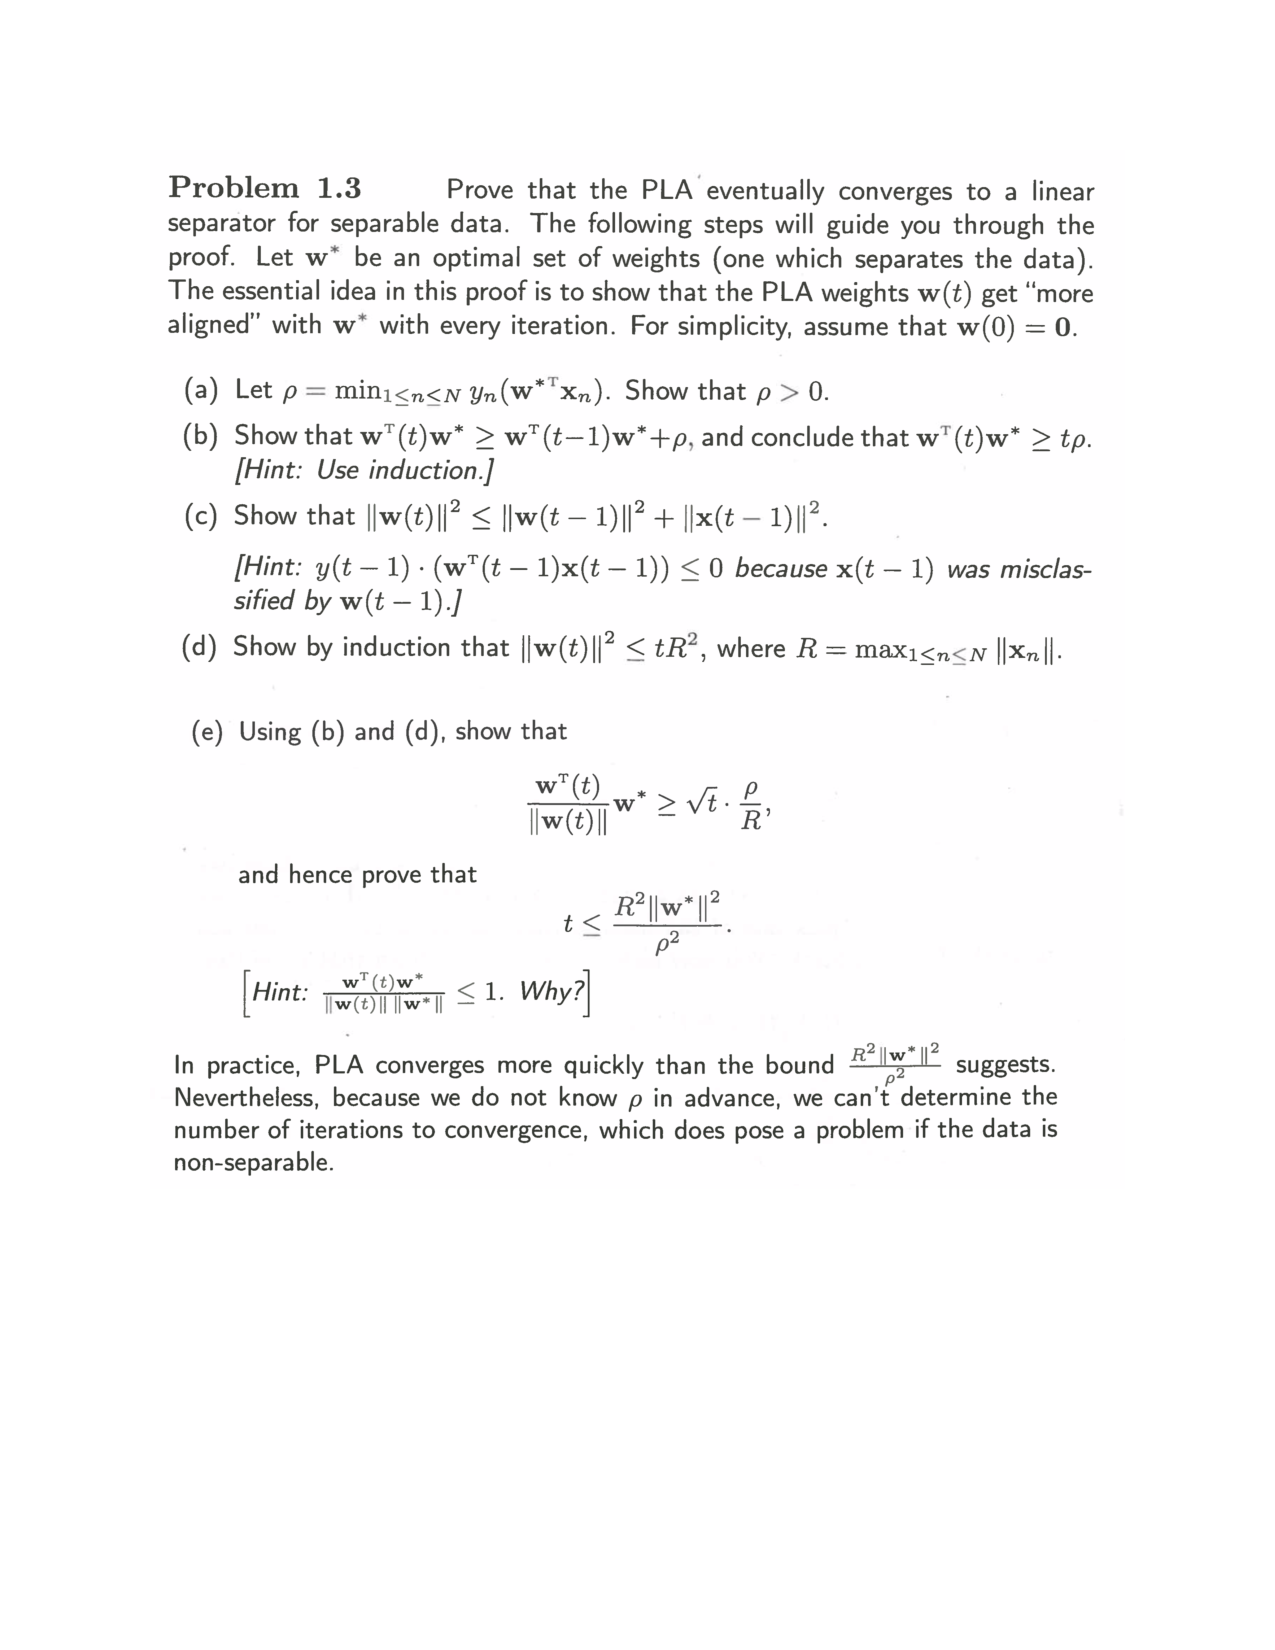
\includegraphics[width=\linewidth]{hw0-q1.pdf}
\end{figure}

\end{document}
